\documentclass[10pt, letterpaper]{article} 

\usepackage{fullpage}
\usepackage[margin=1in]{geometry}
\usepackage{amsfonts, amssymb, amsmath}
\usepackage{tikz,pgfplots}
\usepackage{graphicx}
\usepackage{float}


\def\eq1{y=\dfrac{x}{3x^2+x+1}}

\newcommand{\set}[1] {\setlength\itemsep{#1 em}}

\newcommand\calculator{\tikz{
		\node (c) [inner sep=0pt, draw, fill=black, anchor=south west]{\phantom{N}};
		\begin{scope}[x=(c.south east),y=(c.north west)]    \fill[white] (.1,.7) rectangle (.9,.9);    
		\foreach \x in {.1, .33, .55, .79}{    
		\foreach \y in {.1, .24, .38, .53}{    
		\fill[white] (\x,\y) rectangle +(.11,.07);}} 
		\end{scope} }}
		\def\calcicon#1{\noindent#1 \calculator\ }

\begin{document}
 
\textbf{Questions de pensée critique}

\begin{figure}[H]
\centering
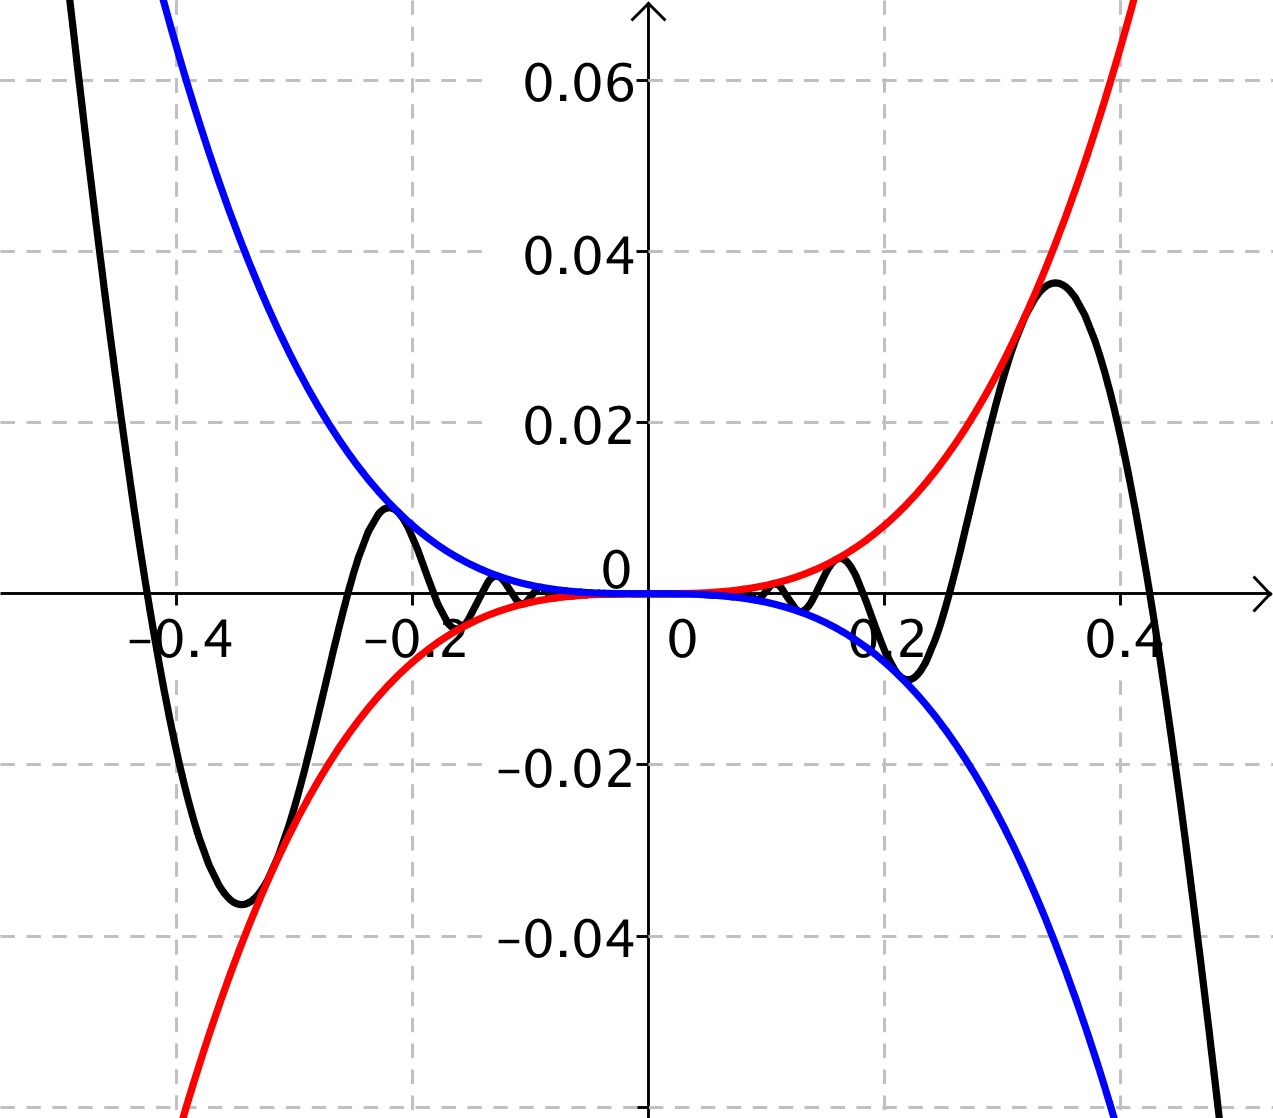
\includegraphics[scale=1, width=0.8\textwidth]{limit}\\
\caption{The Squeeze Theorem}
\end{figure}


\begin{enumerate}
\set{1.2}
\item \calculator\ Examinons la fonction $\eq1$.
\item C'est le symbole de l'ensemble de tous les nombres réels : $\mathbb{R}$.
\item C'est le symbole de l'ensemble des entiers : $\mathbb{Z}$.
\item C'est le symbole de l'ensemble des rationnels : $\mathbb{Q}$.
\item Est-il possible qu'une suite converge vers deux nombres différents ? Si c'est le cas, donnez un exemple. Si non, expliquer pourquoi.
\item Expliquer comment utiliser des sommes partielles pour déterminer si une série converge ou diverge. Donne un exemple
\item Expliquez pourquoi $\int\limits_{1}^{\infty} f(x)\,dx$ et $\sum\limits_{n=1}^{\infty} a_n$ n'ont pas besoin de converger vers la même valeur , même s’ils sont tous deux convergents.
\item Dans vos propres mots, expliquez le théorème des restes de séries alternées. En quoi ce théorème est-il utile ?
\item Expliquez la différence entre la convergence absolue et conditionnelle. Donnez un exemple de chaque.
\item Le test de ratio n'est pas concluant si $\displaystyle{\lim\limits_{n \to \infty} \left| \frac{a_{n+1}}{a_n} \right| =1}$. Donnez un exemple d'une série convergente et d'une série divergente pour lesquelles $\displaystyle{\lim\limits_{n \to \infty} \left| \frac{a_{n+1}}{a_n} \right| =1}$. Expliquez comment vous avez déterminé vos exemples.
\end{enumerate}

\end{document}
​